\section{Effective Practices for Accelerator Design} \label{sec:design}

\subsection{Motivation}
The accelerator design space is vast.  With each new year, many accelerators
are put into products, and even more are proposed through research.  
Table~\ref{tab:overview} highlights just a few of the commercial and 
research accelerators which exist today, in several categories, based around
the program properties they exploit and their hardware mechanisms.
Our research so far
has shown how to take a seemingly impossible task -- comparing and evaluating
accelerators under a common framework -- and made it tractable by providing a
new abstraction.  However, even implementing a TDG-based model for every accelerator
available would be ineffective, due to the effort of testing, validation, etc.
Going beyond the questions of which accelerators are useful, and how do they compare,
is perhaps a more important question: what accelerators would we design for the
next generation of computer architecture?

We broadly outline the impact
of each phase of the current accelerator design process
in Figure~\ref{fig:design-overview}, where the area
of each circular slice indicates the amount of design-space covered in that
phase.  To give more detail, architects first attain insight into possible
accelerator designs using application specific knowledge or analysis of the
inefficiency of general purpose processors.  Analytical models can be
employed, but are generally ineffective because they lack the ability to
comprehend application-accelerator interactions.  Following a high level design
proposal, simulators or simulator extensions are designed and built, while
concurrently either custom microbenchmarks are developed or new compilers are
developed.  Wit some initial version of each, the design
proceeds by modifying the newly developed simulators
and their compilers and running repeated simulations.  After a design is chosen, the
implementation phase begins, either using high-level synthesis tools or lower
level RTL.  Only minor changes in the design can be realistically performed at
this point.  This entire process is repeated for each potential
accelerator design, usually in parallel by separate teams of architects.

\begin{figure}
  \begin{center}
    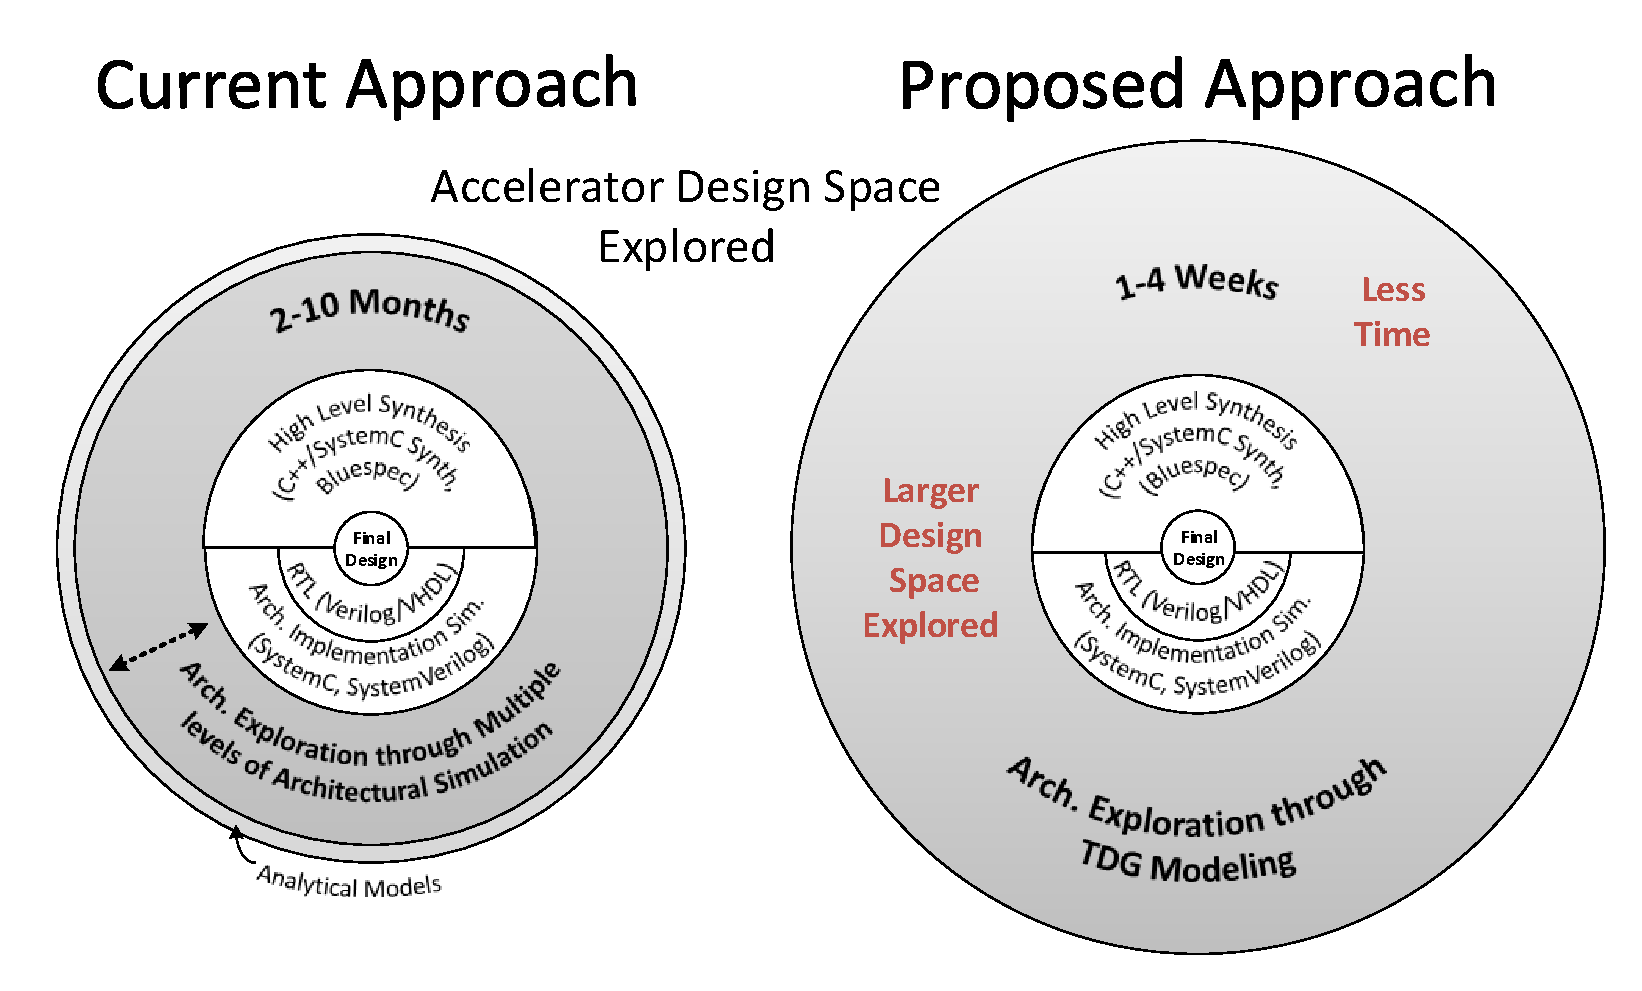
\includegraphics[width=0.8\linewidth]{figs/design-overview.pdf}
  \end{center}
\vspace{-0.2in}
  \caption{Current versus proposed approach for Accelerator Design Practices.}
  \label{fig:design-overview}
\vspace{-0.05in}
\end{figure}

While the above may seem like a natural and plausible strategy, there are
at least three potential pitfalls.

\begin{itemize} 

\item \textbf{Inappropriate Application Binning:} Under the described framework, choosing
the correct set of application domains to target with accelerators is very
difficult.  It becomes easy to \emph{over-design} by binning applications too
aggressively and creating a set of accelerators which does not provide much
benefit over a more conservative set.  It is also easy to \emph{under-design} by
binning too coarsely, and missing out on potential opportunities. 

\item \textbf{Tedious Design Process:}  Designing and implementing
simulators and compilers for each proposed design, along with the
effort of exploring the design space in a simulator model can be tedious.  Part of
the problem is that simulators require a very low-level view of architecture
design.  

\item \textbf{Ignorance of Benefit Overlap:}  Since accelerators are usually designed
in isolation from each other, architects remain unaware of the overlapping benefits
of designs.  Since only one accelerator is active at a time, overlap in benefit
provided is equivalent to wasted designer effort.

\end{itemize}

Overall these pitfalls have the cumulative effect that the design time for the
accelerator is too high, and the design space covered overall is much less. 
This research proposes a design strategy, based on modeling
with the TDG, to aid the early stage design process for accelerators.  
Its aim is to address the above pitfalls of conventional design, 
hastening and broadening design-space exploration, and to
eliminate (or reduce) the need for simulator-based design-space exploration.  
This is shown graphically in Figure~\ref{fig:design-overview}.
This section first describes our methodology,
then present preliminary results in applying
this strategy in designing a particular accelerator.  Both the strategy and
particular designs will be contributions of this work.

\begin{table}
\footnotesize
\def\arraystretch{1.05}
\setlength{\tabcolsep}{.12em}

     \begin{tabular}{>{\RaggedRight}p{0.9in}>{\RaggedRight}p{1.7in}>{\RaggedRight}p{1.7in}>{\RaggedRight}p{2.1in}}  \toprule
    \textbf{Acc-Class} & \textbf{Properties Exploited} &  \textbf{Hardware Strategy} & \textbf{Examples}  \\ \midrule

    Structured Hardware
    & Low-DLP, Mem. Bound Code 
    & Simplified Execution \& Offloading 
    & \textbf{Conservation Cores}~\cite{ccores}, \textbf{BERET}~\cite{Gupta:2011:BER:2155620.2155623}, OptimoDE~\cite{optimoDE}
   \\ 

   SIMD 
   & Regular Data Parallel Code 
   & Parallel Datapath/Vec-Mem Interf.
   & \textbf{SSE}, SODA~\cite{Lin:2006:SLA:1135775.1136494}, VEAL~\cite{VEAL}, Larrabee~\cite{larrabee}, XEON PHI~\cite{chrysos2012intel}
   \\

   CGRAs
   & Computation Pattern Re-use
   & Reconfigurable Datapaths
   & \textbf{DySER}~\cite{hpca2011:dyser}, PIPERENCH~\cite{PipeRench}, CCA~\cite{Clark:2004:APG:1038264.1038929}, FCC~\cite{1629148}
   \\

   Domain Specific
   & Application Specific Behavior
   & Custom Datapaths \& Memory Interfaces
   & HARP~\cite{Wu:2013:NBD:2485922.2485944}, Convolution Engine~\cite{Qadeer:2013:CEB:2485922.2485925}, \textbf{NPU}~\cite{npu}, H.264 Decoding~\cite{Hameed:2010:USI:1815961.1815968}
   \\
    
\bottomrule
  \end{tabular}
  \caption{Accelerator Classes \&  Application/Core Interaction}
  \label{tab:overview}
\vspace{-0.1in}
\end{table}

\subsection{Research Approach} \label{sec:strategy}

The accelerator design strategy we propose contains four phases, and we
describe it below, highlighting how it addresses the pitfalls described
earlier. It bears strong similarities to the existing
practices, which we see as a strong point to its successful adoption.  

%One of the biggest problems with the way accelerator research is done today, is
%that they are designed without respect to whether existing designs can provide
%equivalent benefits.  For instance, an accelerator which provides 2$\times$ benefit
%on a data parallel benchmark which can be accelerated by existing simd techniques
%by $4\times$ is not a figure of merit.  Secondly, architects need a way to quickly
%explore the design spaces to see what potential designs could give enough performance
%and energy benefits to be wroth further lower-level design.
%
%With these insights in mind, we propose the following design strategy.

\begin{enumerate}

\item \textbf{Analysis of Unnaccelerated Regions}  The first step is to use
existing models to automatically find regions which have ``untapped''
potential, and use intuition to find patterns or features of regions which
could be exploited.  That our tool guides architects to unexplored application
domains helps eliminate the improper application-binning pitfall.
(Section~\ref{sec:unexplored})

\item \textbf{High-Level Design Proposal} Using insight from first step, the
second step is to propose a high-level design which can take advantage of
exploitable regions.  Where a conventional high-level design would be defined
merely ``conceptually'' in a typical design process, using our approach, it can
be defined rigorously by creating a TDG transformation which captures the most
essential facets of the architecture.  Since our approach avoids describing
accelerators with ad-hoc simulator models, it helps to reduce the 
pitfall of tediousness of design.  (Section~\ref{sec:hld})

\item \textbf{Design Space Exploration} After enumerating possible design
choices within the high-level design, the third step is performing design space
exploration using TDG modeling to find the simplest design that meets
performance/energy targets.  Because our methodology allows us to keep multiple
accelerator models in the same evaluation framework, it remains easy to
determine if accelerators are providing overlapping benefit, which helps
prevent this pitfall. Also, the analysis or ``meta-information'' gathering
component to the TDG acts as an optimistic compiler, allowing the designer
to separate software and hardware concerns. (Section~\ref{sec:design-space})

\item \textbf{Design Refinement} The final step is to
iteratively refine the design by developing
concrete mechanisms and update the TDG model.  The tediousness of design
is also reduced in this stage because of the employment of high-level models
which can be iteratively added to.
(Currently Proposed Work)

\end{enumerate}
%First, in section~\ref{sec:unexplored} 
%we show there are yet-unexplored opportunities for acceleration for a 
%variety of program region types, using the existing models as a guideline 
%for what can already be accelerated effectively, and what can't.  
%Second, in Section~\ref{sec:nla},
%using this insight, we will present different high-level designs 
%for an accelerator, specifically one which exploits nested loop program structures,
%along with clustered computations, and discuss the potential benefits of
%these designs.


\subsection{Preliminary Results} 

In this section, we describe the process and benefits of our
proposed design strategy in more detail by applying it to a specific design.
Both the specific designs which we deliver, as well as the design process,
will be contributions of this proposed work.

\subsubsection{Analysis of Unnaccelerated Regions} \label{sec:unexplored}

%\label{sec:unexplored}
%To get insight into the acceleration opportunities of the future, one must
%first understand when and why the existing designs are ineffective.
%Modeling all accelerators is impossible, so the approach we take is
%to model accelerators which exploit a spectrum of various program properties and
%use different micro-architectural mechanisms.  Table~\ref{tab:overview} how
%the accelerators we target, shown in bold, straddle a significant portion of
%the accelerator space.  

Using TDG models, it becomes possible to analyze a program in a
region-by-region fashion, to find those regions which cannot be accelerated by
the existing models, or which have significant potential.  
We use the methodology below to analyze these regions, and
then we determine the reasons which they are not accelerated.

\paragraph{Methodology} The regions we consider, from smallest to largest granularity,
are traces, inner loops, outer loops, and whole functions.  To be clear, every cycle
of the program is accounted for by some region. We run our models on 
the benchmarks described in the previous section (SPEC,Mediabench,Parboil,Intel TPT), 
and with the DySER, SIMD, BERET, and CCores models.  For the purposes of this study, 
we consider a region to be ``unaccelerated'' when the degree of speedup attained is
less than 30\%.  For providing broad insights, we classify unaccelerated regions
through manual inspection of their associated source code 
into five categories, which we describe below.

\begin{itemize}[itemsep=0.5pt, topsep=8pt, partopsep=0pt]
  \item \textbf{Memory Latency Bound} These regions exhibit indirect memory access,
like tree traversal or pointer chasing.  Because the computation for these regions is
generally very lightweight, accelerators should likely remain as simple as possible, while
achieving the same performance as the baseline core.
  \item \textbf{Loop Parallel + Irregular Memory} These regions exhibit significant loop 
parallelism, but are ineffective for architectures which exploit vectorization, because
memory access must be performed in a scalar fashion.  The best way to target these architectures may be through scatter gather techniques. 
  \item \textbf{Excess Accelerator Serialization} These regions are characterized by
excess control flow, making them ineffective for vectorization, or by significant
memory access, which tends to serialize the structured hardware accelerators which
we considered.  
  \item \textbf{Accelerator Incompatible}  These regions are those which are incompatible
with the set of accelerators we have, because the target certain program structures.
These include nested loops, short-but-frequent functions, and recursive functions.
  \item \textbf{Other}  This category is a catchall for regions which have more complex
interactions which could not be precisely determined, or if the corresponding
 source was unavailable.
\end{itemize}

\begin{figure}
  \begin{center}
    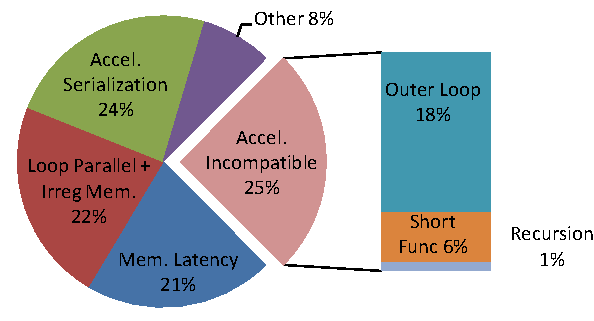
\includegraphics[width=0.55\linewidth]{figs/unacceleratable_regions.pdf}
  \end{center}
\vspace{-0.2in}
  \caption{Breakdown of Unnacceleratable Regions (those which have $<30\%$ performance improvement)}
  \label{fig:unacc}
\vspace{-0.05in}
\end{figure}

\paragraph{Analysis}  Our first result is that
50\% of the program's regions, in terms of their contribution to
the overall execution time, cannot be accelerated by given accelerators.
This suggests that there may be ample opportunity for new accelerator designs.  To go
more in depth, Figure~\ref{fig:unacc} shows the breakdown of various regions types
with the above categorizations, for which there were 73 regions.

Roughly equal portions of the programs execution fall
into the above four categories.  First, the fact that many of the unacceleratable 
regions are attributable to high memory latency and irregular memory in loop parallel
regions, means that extremely simple accelerators and scatter/gather extensions to
SIMD are indeed of significant value.  Also, many of the regions fall
into the excess accelerator serialization category, meaning that too much control
or memory access is preventing them from reaching better performance than the OOO core.
Most interestingly, however, is the fact that many regions are not able to be
accelerated because of the program structures which are used, and specifically outer
loops seem to pose the most impactful problem.

\paragraph{Program Structure Breakdown}
To shed more light on the various program structures used in programs, 
Figure~\ref{fig:region-type} categorizes every dynamic instruction
into one of several categories: \emph{hot traces} which are single
paths through inner loops, \emph{flat inner loops} which are inner loops with no function
call boundaries, \emph{inner loops}, \emph{any loop} which includes all forms of nested
natural loops, \emph{direct recursion} from one function to itself, and \emph{any recursion}.  The remainder of dynamic instructions are those which occur in functions while
not in a loop or recursion, typically because of many repeated calls.

As Figure~\ref{fig:region-type} shows, the program structure types vary
significantly by program, but on average hot traces are very common, about 57\%
of the dynamic execution.  Most interesting is that, on average, more than 20\% of the
dynamic instructions happen inside more general loops structures.  On current
accelerators, these instructions cannot be efficiently executed.

\begin{figure}
  \begin{center}
    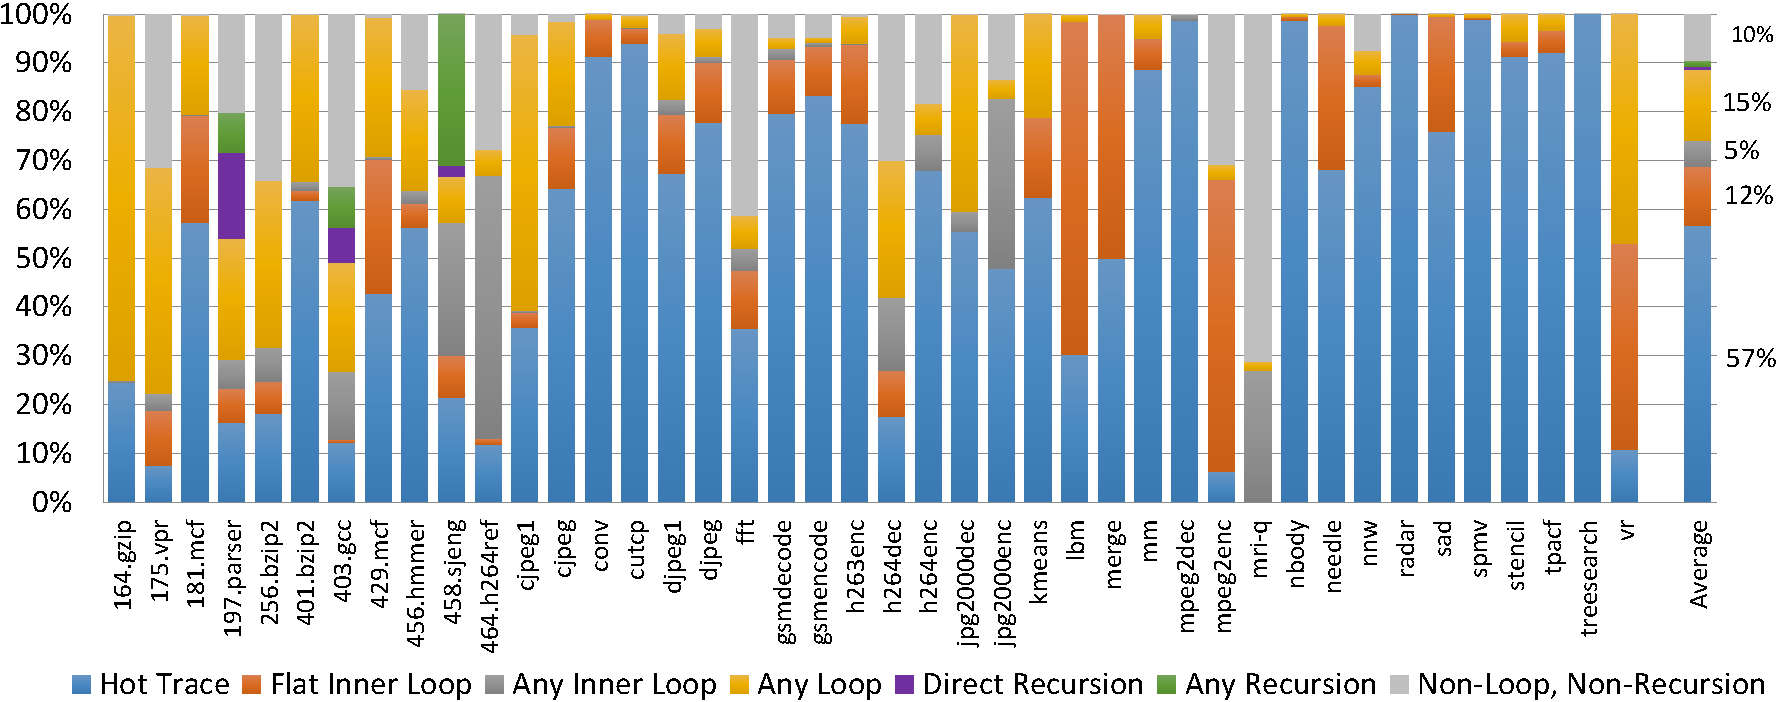
\includegraphics[width=1.0\linewidth]{figs/region-type.pdf}
  \end{center}
\vspace{-0.2in}
  \caption{Program structure break down in percentage of dynamic instructions.}
  \label{fig:region-type}
\vspace{-0.05in}
\end{figure}

\subsubsection{High Level Design: Nested Loop Accelerator (NLA)} \label{sec:hld}
To demonstrate the ability of the TDG to perform the high-level design tradeoffs
for new architectures, we pick a specific ``domain'' and architectural style.  
Leveraging the insights that nested-loops are important across many benchmarks, 
are exploitable and are under-targeted in existing accelerator designs, we will focus 
on them here.  We also need to choose some basic aspects of the architecture
to guide the exploration.  Using the insight from the limit study in section 2,
reconfigurable hardware accelerators can provide significant energy-efficiency
benefit.  We choose to explore clustered-instruction execution, like that of
BERET rather than the more grid-style fabric of DySER, as the latency of computation
will be more important for non-DLP codes which we target here.

We briefly elaborate on the hypothetical architecture and compiler design, 
and then describe how the new accelerator's design space can 
be modeled and explored using the TDG.

\paragraph{Hardware Overview}

Fundamentally speaking, NLA is an in-core accelerator, based on clustered functional
unit computation, targeting general purpose execution of nested-loops.  It can
take full control from the main processor when the region is entered, and returns
control when the region is complete, transferring state to and from the processor's
register file on the transfer of execution.   It achieves energy efficiency through
the compound functional units which can eschew register file access, and by not
requiring frontend pipeline stages (fetch/decode/rename/dispatch) on each instruction.
Figure~\ref{fig:nla-arch} shows a hypothetical block diagram for NLA with many design
aspects left undecided.  Some examples are, ``should NLA communicate through
a centralized register file, or should state be distributed?'',  or ``should NLA allow
multiple memory requests through an LSQ-like structure, or should it serialize and 
just use a simple store buffer.''  
A later section organizes these into specific design points.

%Later in this section, organize a few of these
%questions into more specific design points which we model and discuss in more detail.

\begin{figure}
  \begin{center}
    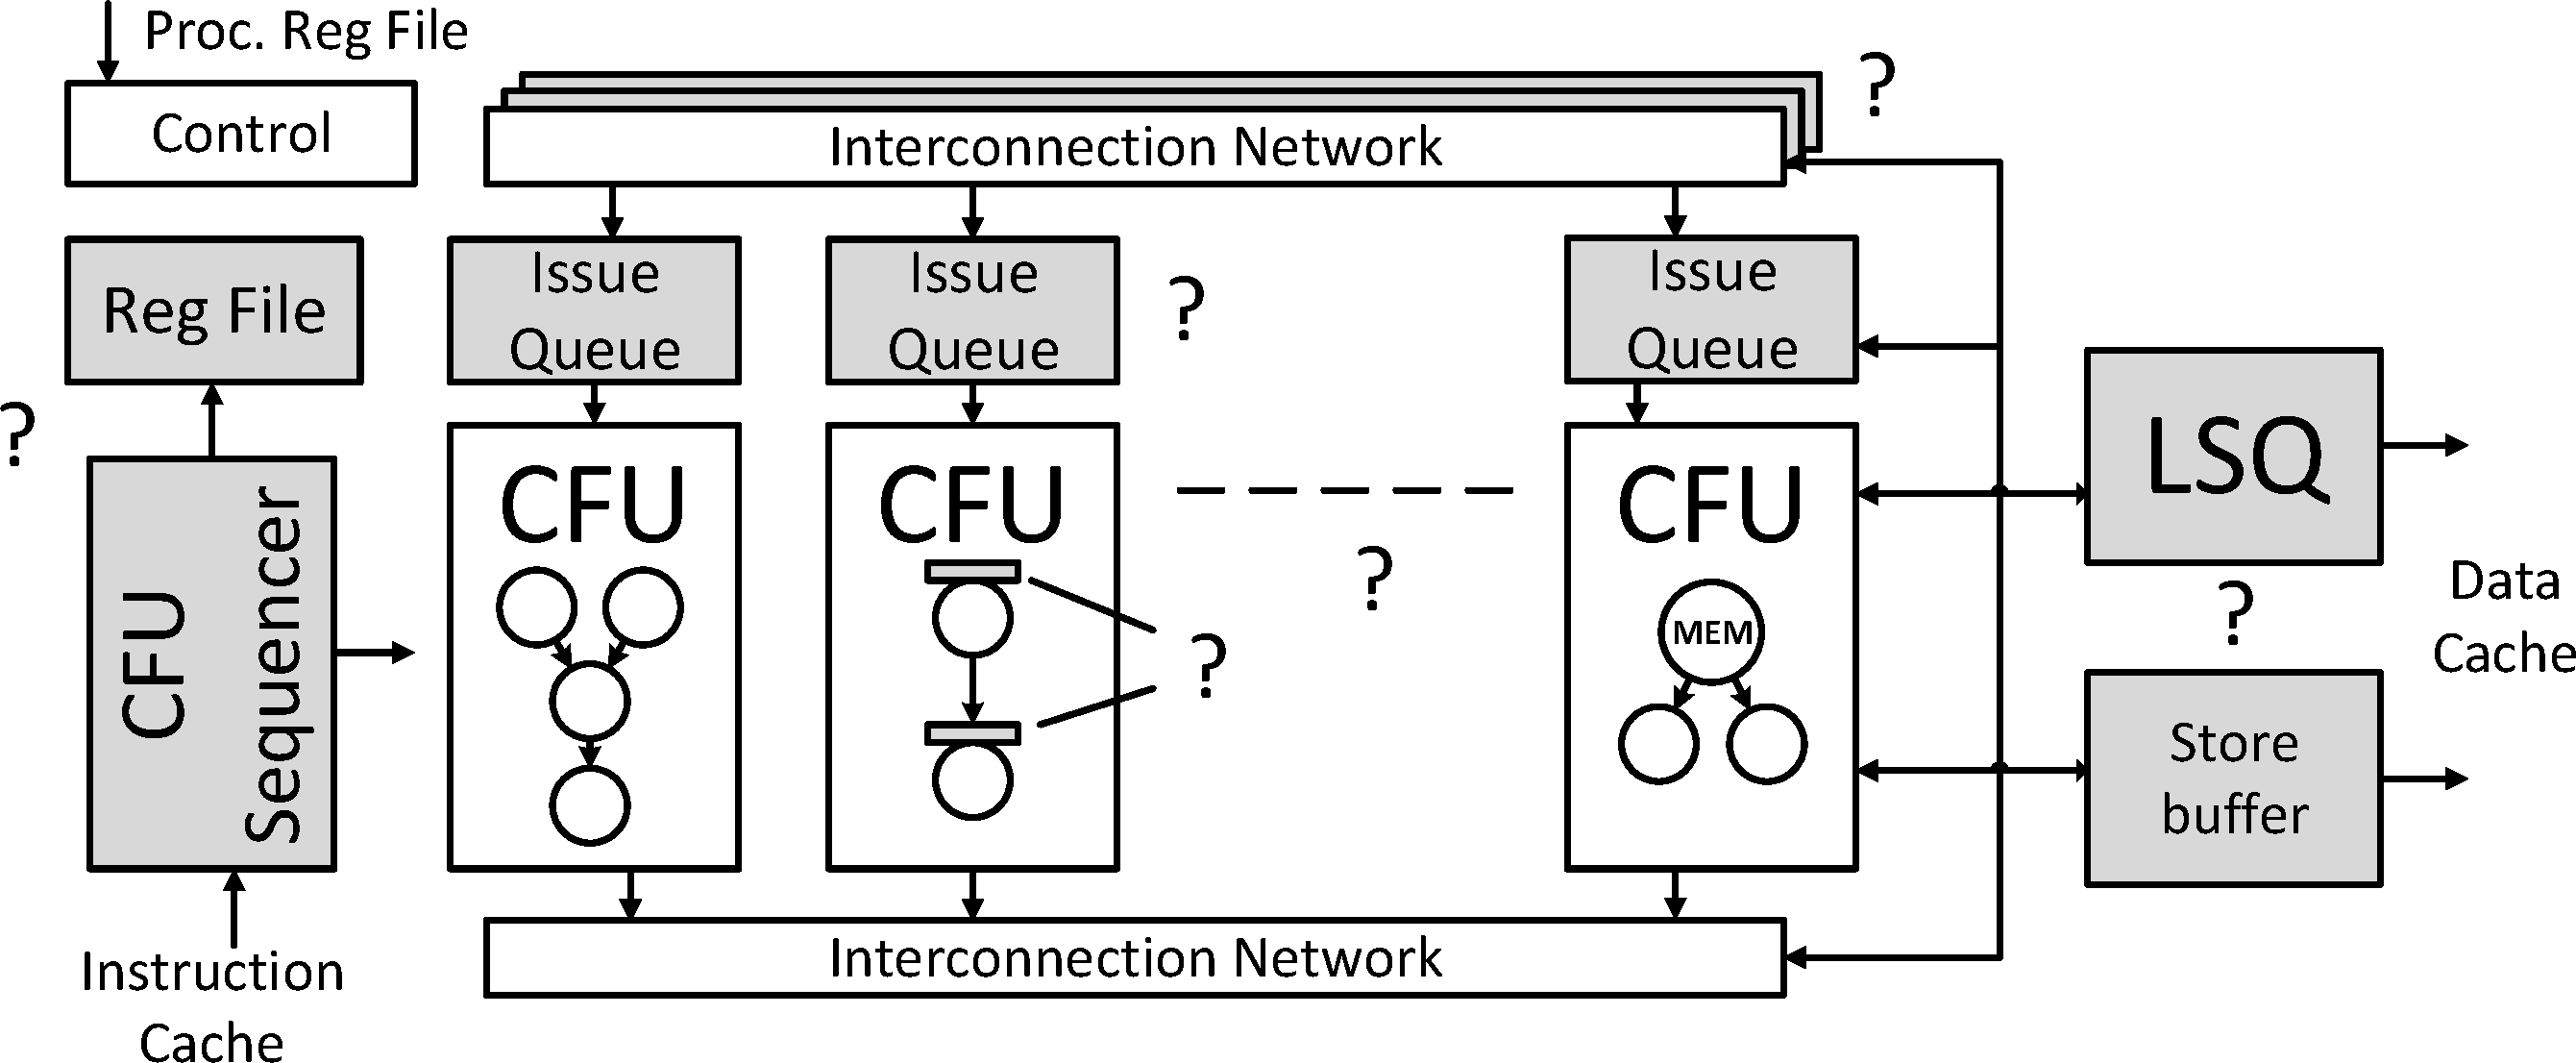
\includegraphics[width=0.85\linewidth]{figs/nla-arch.pdf}
  \end{center}
\vspace{-0.2in}
  \caption{Hardware architecture for NLA accelerator.  ``?'' show potential high-level design decisions.}
  \label{fig:nla-arch}
\vspace{-0.05in}
\end{figure}


\paragraph{Gathering NLA Meta-information}
To use our framework to evaluate an architecture, we need to consider a hypothetical
compiler design, which we refer to as ``gathering meta-information.''  
The most important concern for a clustered-FU accelerator is how to partition the
instructions onto the various compound FUs.  This somewhat resembles the spatial 
architecture scheduling problem of~\cite{ILP_Sched}, and we use parts of the solution
for our initial NLA scheduler

We briefly formally describe the NLA scheduling problem, and present a simple
integer linear program (ILP) to solve it.  Consider a computation graph made of
vertices $v \in V$, where $G_{v_{1}v_{2}}$ represents data dependences between
vertices $v_1$ and $v_2$.  Similarly, consider a hardware graph of computational
resources $n \in N$, where $H_{n_{1}n_2}$ represents the connections of the
hardware substrate between $n_1$ and $n_2$.  The compatibility between hardware
resources and computation vertices 
is given by the set $C_{vn}$.  The goal is to attain a mapping
$M_{vn}$ from computation vertices to hardware nodes such that the number of
edges in $G$ not mapped to edges in $H$ is minimized, essentially minimizing
the interconnection network traffic between compound FUs.  We give the ILP to
solve this problem in Table~\ref{tab:nlasched}.  Proposed work describes
making this solution even more general and aggressive.
In general, integer linear programming is a good fit for an optimistic
compiler, as it can guarantee important solution properties. 



\begin{table*}[h]
\begin{center}
\setlength{\tabcolsep}{.18em}
\def\arraystretch{1.3}
\small 
\begin{tabular}{m{0.5\linewidth}m{0.5\linewidth}}

\multicolumn{1}{c}{\textbf{ILP Equation}} & \multicolumn{1}{c}{\textbf{Explanation}} \\
\toprule

\centering
$\forall_{v\in V} \sum_{\substack{n \in C_{vn}}} M_{vn} = 1 $

$\forall_{v\in V} \sum_{n \notin C_{vn}} M_{vn} = 0$
& These equations enforce that all computational vertices are mapped to exactly
one compatible node.
\\ \midrule

\centering
\begin{eqnarray*}
\Forall_{\substack{ \\v_1v_2 \in G \\ n \in N}}
  B_{v_{1}v_2} \ge  M_{v_{2}n_2} - \sum_{\substack{n_1 \in C_{v_{1}n_1}\\ n_1n_2 \in H}} M_{v_{1}n_{1}}  
%         Bvv(v1,v2) =g= -sum(fu1$(c(v1,fu1) and Hnn(fu1,fu2)),Mvn(v1,fu1)) + Mvn(v2,fu2);
\end{eqnarray*}

& This constraint computes a set of binary variables $B_{v_{1}v_2}$ which describe 
whether two computation vertices map to the same node.  If $B$ is false, then
there is no ``boundary'' between the nodes, and they execute in the same instance 
of a CFU. 
\\ \midrule

\centering
\begin{eqnarray*}
\Forall_{v_1,v_2,v_3 \in P_{v_{1}v_{2}v_{3}} } 
  (1-B_{v_{1}v_{2}}) + (1-B_{v_{2}v_3}) -1 \le (1-B_{v_{1}v_3}) 
\end{eqnarray*}

& This constraint enforces boundary transitivity: if there is no boundary between
$v_1$ and $v_2$, and there is no boundary between $v_2$ and $v_3$, then there
can't be a boundary between $v_1$ and $v_3$.  It uses the set $P$, which
contains members of $V$ which are possible to map to each-other, which is
computed offline using a simple graph traversal.  
\\ \midrule

\centering
$\Forall_{v_1,v_2,n \in C_{v_{1}n} \cap C_{v_{2}n} \cap P_{v_{1}v_{2}} }
M_{v_{1}n} + M_{v_{2}n} \le B{v_{1}v_{2}} +1$

& This constraint makes sure that two nodes which could possibly map to each other, are 
only allowed to map to the same hardware node if they are on the same CFU. 
\\ \midrule

\centering
$ R = \sum_{v_{1},v_{2} \in G} B{v_{1}v_{2}}$

& This equation defines $R$, the number of either register file reads, or interconnection
network accesses.  $R$ is the objective of minimization.


\\ \bottomrule

\end{tabular}

\caption{Integer linear programming model for NLA Scheduling.}
\label{tab:nlasched}  
\end{center}
\vspace{-0.15in}

\end{table*}





\if 0
binary variable Mvn(v,n), Bvv(v,v);
positive variable Tv(v);

%not sure if i need this
%route1(v1,v2,fu2)$(A(v1,v2) and c(v2,fu2)).. 
%      Mvn(v2,fu2) =l= sum(n1$(c(v1,n1) and Hnn(n1,fu2)), Mvn(v1,n1));

boundary(v1,v2,fu2)$(A(v1,v2) and c(v2,fu2))..
         Bvv(v1,v2) =g= -sum(fu1$(c(v1,fu1) and Hnn(fu1,fu2)),Mvn(v1,fu1)) + Mvn(v2,fu2);

transitive_sameness1(v1,v2,v3)$(ORD(v1) lt ORD(v2) and ORD(v2) lt ORD(v3) and
                              close_dep(v1,v2) and close_dep(v2,v3) and close_dep(v1,v3))..
                              (1-Bvv(v1,v2)) + (1-Bvv(v2,v3)) -1 =l= (1-Bvv(v1,v3));

* Enforce that !Bvv(v1,v2) -> M(v,fu1), M(v,fu2) fu1!=fu2
restrict_fu(v1,v2,fu)$(c(v1,fu) and c(v2,fu) and (ORD(v1) lt ORD(v2)) and possDep(v1,v2))..
                              Mvn(v1,fu) + Mvn(v2,fu) =l= Bvv(v1,v2) +1;


timing1(v1,v2)$(A(v1,v2)).. Tv(v2) =g= Bvv(v1,v2) + Tv(v1);
timing2(v1,v2)$(A(v1,v2)).. Tv(v2) =l= 20*Bvv(v1,v2) + Tv(v1);

c_reads..  READS  =e= sum((v1,v2)$(A(v1,v2)), Bvv(v1,v2));
\fi


\subsubsection{Design Space Exploration} \label{sec:design-space}

Table~\ref{tab:nlatrans} below describes four NLA design points, from most simplistic
and presumably energy-efficient, to most complex and high-performance.  The basic
hardware required is briefly described in the first column, and the second column
describes the TDG transformations required to model these mechanisms, or hypothetical
features.  Note that there is a close correspondence between hardware mechanism and
dependence graph transform, enabling very fast exploration of architectural designs.
This setup is related to and inspired from the limit relaxations in the
previous section.  The difference here is that, while we only show four designs 
for brevity, in general, the cross product of possible design 
decision/graph transformations are useful and interesting for the designer, and will
be evaluated.

In our design space exploration, in addition to evaluating NLA's design points,
we also evaluate existing accelerators.  In Figure~\ref{fig:nla-prelim} we show
preliminary results for six of the benchmarks from PARBOIL and TPT benchmark
suites, using the four design points described earlier.  The first two
benchmarks, cutcp and mm, exhibit accelerator benefit overlap with all NLA
designs, because either SIMD or DySER is more effective, even for the most
aggressive NLA designs.  For the second two benchmarks, nnw and merge, for all but
the most aggressive speculative-OOO version, NLA's benefit is masked by other
accelerators.  For these four benchmarks, we no longer need to consider NLA as a potential
accelerator design.  Looking at the last two benchmarks, tpacf and lbm, the practical
NLA-decoupled design actually performs well compared to the other accelerators and the
general purpose processor.  Finally, we can also observe than the sequential and 
pipelined designs are ineffective for competing with an OOO core.

Overall these experiments have shown how we can eliminate potential designs and
many benchmarks from consideration, all with the use of extremely high level
models and low design-effort.  Also, though we have only shown four design points for
the sake of brevity, we can make and evaluate design choices independently, so
we can explore many more designs very rapidly.

\begin{figure}
\begin{center}
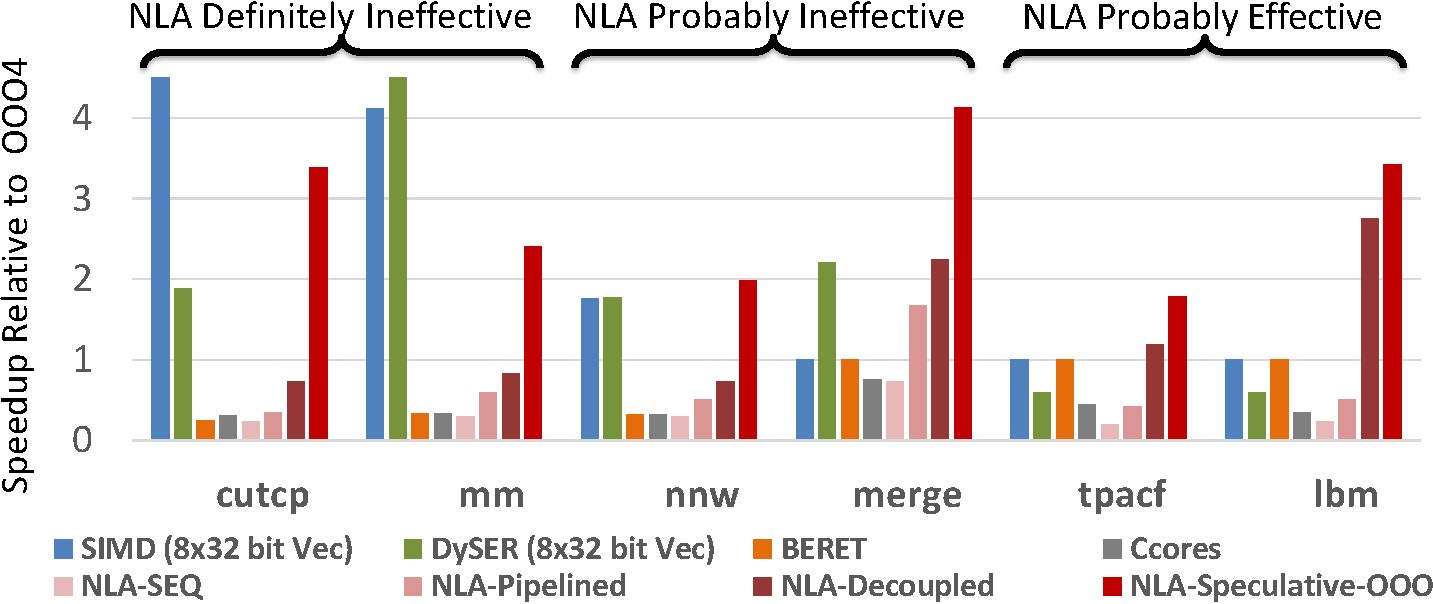
\includegraphics[width=0.68\linewidth]{figs/nla-results-slide.pdf} 
\end{center}
\vspace{-0.1in}
\caption{Preliminary Results for NLA-Design Space Exploration}
\label{fig:nla-prelim}
\end{figure}

\begin{table*}[h]
\begin{adjustwidth}{-0.6in}{-0.6in}
\begin{center}
\setlength{\tabcolsep}{.18em}
\def\arraystretch{0.0}
\footnotesize 
\begin{tabular}{m{0.01\linewidth}@{}m{0.48\linewidth}m{0.48\linewidth}}

Design Point
& \multicolumn{1}{c}{\textbf{Hardware Implications}}
& \multicolumn{1}{c}{\textbf{TDG Transformations}}
\\   \midrule

\parbox[t]{3mm}{\hspace{0.1in}\rotatebox[origin=c]{90}{\textbf{Serialized}}} 
& 
\begin{itemize}
%\item \textbf{CFG\&DFG}
\item \textbf{} Serialized hardware implies simple design, no arbitration need.
\item \textbf{} Regfile stores results bet wen each invocation.
\item \textbf{} Forwarding network for passing values used by subsequent instructions.
\end{itemize}


& 
\begin{itemize}
\item \textbf{} Edges inserted between the end and beginning of subsequent CFU nodes.
\item \textbf{} Dependence inserted between memory address calculations in program order.
\end{itemize}
\\ [-0.6\normalbaselineskip]  \midrule

\parbox[t]{1mm}{\rotatebox[origin=c]{90}{\textbf{Pipelined}}} 
& 
\begin{itemize}
\item \textbf{} On each cycle, Sequence Unit issues the next compound instruction if its operands are ready and CFU is not busy.
\item \textbf{} Writeback bus must be arbitrated so only one CFU can write at a time.
\end{itemize}
&
\begin{itemize}
\item \textbf{} Edges are inserted between the CFU invocations.
\item \textbf{} Control operations serialize the next CFU invocation.
\item \textbf{} CFUs are treated like resources, and dynamic edges are added between nodes
requesting contended CFUs.
\end{itemize}

\\ [-0.6\normalbaselineskip]  \midrule

 
\parbox[t]{1mm}{\rotatebox[origin=c]{90}{\textbf{Decoupled}}} 
& 
\begin{itemize}
  \item \textbf{} Dataflow architecture with distributed issue queues across CFUs.  Issue queues fire when operands are ready and CFU is free.
  \item \textbf{} Software disambiguates the memory addresses by static load/store where possible, unknown accesses are serialized.
  \item \textbf{} Interconnection network is multi-issue point to point.
  \item \textbf{} CFUs are pipelined for additional parallelism.
\end{itemize}

&
\begin{itemize}
\item \textbf{}Only CFU serialization edge is for enforcing control dependence.
\item \textbf{}Edges inserted only between memory-operations which may alias through
software analysis.
\item \textbf{}Interconnection bus treated as resource, dynamic edges inserted during
contention.
\end{itemize}
\\  [-0.6\normalbaselineskip] \midrule


\parbox[t]{1mm}{\rotatebox[origin=c]{90}{\textbf{Spec. OOO}}} 
&
  \begin{itemize}
  \item \textbf{}Full speculative support allowing execution past control
nodes.
  \item \textbf{}Mispeculated instructions squashed.  (hypothetical mechanism)
  \item \textbf{}Memory dependence prediction.  (hypothetical mechanism)
  \end{itemize}
&
  \begin{itemize}
  \item \textbf{}No CFU serialization edges.
  \item \textbf{}Squash penalty enforced by multi-cycle dependence between complete of mis-speculated control and subsequent instruction.
  \item \textbf{}Squash penalty inserted for mispeculated memory dep prediction.
  \end{itemize}
 
\\ [-0.6\normalbaselineskip]  \bottomrule 

\end{tabular}

\caption{Description of NLA Design Points and their Models}
\label{tab:nlatrans}  
\end{center}
\vspace{-0.15in}
\end{adjustwidth}

\end{table*}


\subsection{Proposed Work} The proposed work falls into several categories.
For the NLA accelerator, there is essentially work left in the
third and fourth design phases.  We also will explore two more-speculative ideas.

\paragraph{Exploration Phase} The exploration space should be increased in terms of
architectural features.  Also, running a larger, more representative set of
benchmarks will be necessary.  On the compiler side, it can be extended in a
variety of potentially useful ways.  The scheduling problem, as described
earlier, can only minimize the network activity, and
 does not attempt to optimize latency or throughput by considering the
utilization/contention of resources.  Attempts to model these features
have so far produced integer linear programs which are too slow.  The
proposed work will explore whether ILP for more aggressive scheduling is
possible.

\paragraph{Refinement Phase} 
To complete step 4 of the accelerator design strategy outlined earlier,
we will iteratively design the ``low-level'' hardware features.  
For example, protocols for handling full buffers in the dataflow 
network, which can prevent deadlock and allow forward progress, are necessary.  Another
example would be the mechanism which forwards the memory access token between
memory which may alias.  Once mechanisms are decided upon, then dependence nodes
and edges for these features can be added, and more realistic models can be attained.

\paragraph{Automating Analysis}
One of the most pressing issues is in how to give more insight to the designer 
to inspire interesting and useful accelerator designs, as well as insight to why
certain designs are better than others.  One possibility is to characterize 
``unexplored'' or ``high-benefit'' applications automatically into groups based on
certain observed program characteristics, in an attempt to make analysis easier.  
Clustering algorithms may be able to be employed for this purpose.  
Another useful feature would be in understanding fundamentally why certain designs
or design variations perform differently.  One possibility is to use the critical
path through the graph to see what dependency types are most prevalent in a certain
execution.  By associating dependency types with architectural features, we should be
able to discern what is the prevailing cause for various speedups and slowdowns.

\paragraph{Further Accelerator Designs} Finally, in
Section~\ref{sec:unexplored} we discovered several categories of program
regions which go unaccelerated in important applications.  Part of this
dissertation will explore whether there are further opportunities for new
acceleration paradigms. 

Also, it is important for evaluating the design process to
isolate the benefits of the particular design we target with 
the benefits design process itself.  One way to do this would be to 
re-design an accelerator which we have developed using standard
practices, then qualitatively compare the difficulties of each approach,
and quantitatively compare the design quality.  One possibility is
to use our research group's ``MAD'' accelerator.


\subsection{Related Work} 

\paragraph{ADLs for Compiler/Architecture/Simulator Generation} One body of
particularly related work uses architecture description languages (ADLs) as a
specification tool for rapid architectural exploration and evaluation.
UPFAST is a tool for generating a simulator and assembler/disassembler,
mainly used for extensions to MIPS-based architectures~\cite{upfast}.
BUILDABONG is a tool for architecture compiler co-exploration, requiring
architectural specification with an abstract state machine, and can generate
HDL models, simulators and compilers~\cite{build_a_bong}.  Productized
approaches include the Tensilica Instruction Extension language
~\cite{Gonzalez:2000:XCE:623292.624348}, which allows for the manual creation
of specific instructions which can be automatically incorporated into
existing architectures and compilers. For a comprehensive survey on
automatic instruction-set extensions, see Galuzzi et
al.~\cite{Galuzzi:2011:IEP:1968502.1968509}. Another example is the Language
for Instruction Set Architectures (LISA)~\cite{Hoffmann:2002:AEE:640673},
which can be used to generate compilers, assemblers and functional
simulators, as well as hardware implementations.  

%To further automate this process,
%Tensilica's ``Xpres compiler'' and Synopsys's ``Processor Designer'' take as
%input an application written in C, and produce highly customized processors
%with application specific instructions.  

The Liberty Simulation Environment~\cite{vachharajani2006liberty} is a somewhat
unique tool which can be used to create simulation models which are more
accurate, and as the authors claim, more intuitive and maintainable than those
created using sequential languages.  A language called the Liberty Structural
Specification~\cite{liberty} is used to construct
models of hardware components which are connected through explicitly defined
interfaces, rather than the implicit interfaces of the function-abstractions
which sequential languages provide. 

While the above approaches can aid the design, exploration and even generation
of architectures, simulators and compilers, they are only applicable for certain
types of instruction-by-instruction, Von Neumann style architectures.  For accelerator
design, we need something more general and powerful.

\paragraph{High Level Synthesis} High-Level Synthesis (HLS) attacks design
inefficiency from the bottom up: its goal is to make the development of
hardware designs easier by using languages which are higher level than either
Verilog or VHDL.  Typically, these tools take hardware designs written in
high level languages like C,C++ or SystemC, and produce optimized,
synthesizable RTL~\cite{5209959}.  Because sequential languages aren't
necessarily effective for expressing hardware designs, another HLS tool,
Bluespec~\cite{bluespec}, uses a custom language based on Haskell and
SystemVerilog.  

We see our proposed approach as being largely compatible with HLS tools,
which can take over to explore more fine-grained, implementation-specific
tradeoffs after the broad design-space exploration that our approach allows.

\paragraph{Accelerator Design Processes} In terms of accelerator design
strategies, we are certainly not the first to recognize that designing for
multiple accelerator systems are important.  The most closely related
strategy is the 10$\times$10 framework~\cite{10by10}.  Their essential
strategy is to describe clusters of applications which exhibit certain
behaviors, and develop in-core ``micro-engines'' (accelerators) which target
each domain.  The key difference between our approaches is that they separate
and delineate benchmarks into categories \emph{a priori}, while our approach
can find patterns across predefined benchmark ``categories,'' and therefore
can find a more optimal, and likely more lean set of accelerators.

\paragraph{Architecture}
In terms of the hardware design, NLA borrows many concepts from the BERET
architecture~\cite{Gupta:2011:BER:2155620.2155623}.  However, it's prospective
design and intended purpose differ in several key aspects.  First, it targets
nested loops, which are much more general than the hot-traces which BERET
targets, and allows for longer accelerator-only periods where the core can
enter into lower power states.  Also, it has the potential to deserialize
aspects of the execution which would can lead to performance levels useful
in OOO processors.
